\documentclass{standalone}
\usepackage{tikz}
\usetikzlibrary{patterns, positioning}

\begin{document}
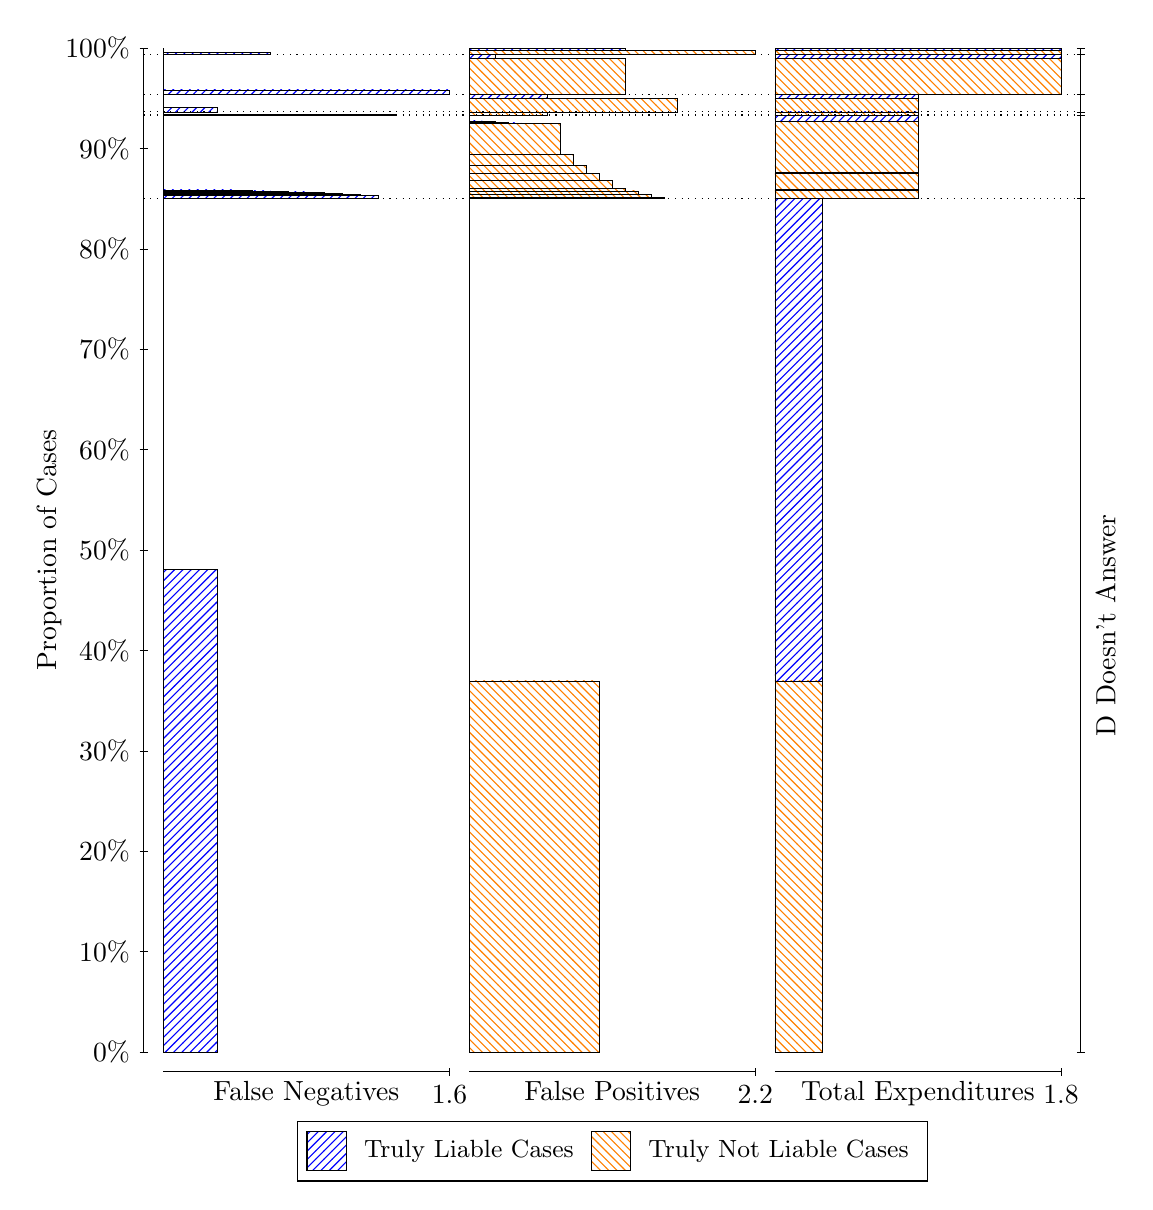
\begin{tikzpicture}
\draw[black, very thin] (1.5,1.75) -- (1.5,14.5);
\node[rotate=90, anchor=center] at (0.3, 8.125) {Proportion of Cases};
\draw[black, very thin] (1.45,1.75) -- (1.55,1.75);
\node[anchor=east] at (1.45, 1.75) {0\%};
\draw[black, very thin] (1.45,3.025) -- (1.55,3.025);
\node[anchor=east] at (1.45, 3.025) {10\%};
\draw[black, very thin] (1.45,4.3) -- (1.55,4.3);
\node[anchor=east] at (1.45, 4.3) {20\%};
\draw[black, very thin] (1.45,5.575) -- (1.55,5.575);
\node[anchor=east] at (1.45, 5.575) {30\%};
\draw[black, very thin] (1.45,6.85) -- (1.55,6.85);
\node[anchor=east] at (1.45, 6.85) {40\%};
\draw[black, very thin] (1.45,8.125) -- (1.55,8.125);
\node[anchor=east] at (1.45, 8.125) {50\%};
\draw[black, very thin] (1.45,9.4) -- (1.55,9.4);
\node[anchor=east] at (1.45, 9.4) {60\%};
\draw[black, very thin] (1.45,10.675) -- (1.55,10.675);
\node[anchor=east] at (1.45, 10.675) {70\%};
\draw[black, very thin] (1.45,11.95) -- (1.55,11.95);
\node[anchor=east] at (1.45, 11.95) {80\%};
\draw[black, very thin] (1.45,13.225) -- (1.55,13.225);
\node[anchor=east] at (1.45, 13.225) {90\%};
\draw[black, very thin] (1.45,14.5) -- (1.55,14.5);
\node[anchor=east] at (1.45, 14.5) {100\%};

\draw[black, very thin] (13.4,1.75) -- (13.4,14.5);
\draw[black, very thin] (13.35,1.75) -- (13.45,1.75);
\node[anchor=west] at (13.35, 1.75) {};
\draw[black, very thin] (13.35,12.589) -- (13.45,12.589);
\node[anchor=west] at (13.35, 12.589) {};
\draw[black, very thin] (13.35,13.649) -- (13.45,13.649);
\node[anchor=west] at (13.35, 13.649) {};
\draw[black, very thin] (13.35,13.689) -- (13.45,13.689);
\node[anchor=west] at (13.35, 13.689) {};
\draw[black, very thin] (13.35,13.915) -- (13.45,13.915);
\node[anchor=west] at (13.35, 13.915) {};
\draw[black, very thin] (13.35,14.42) -- (13.45,14.42);
\node[anchor=west] at (13.35, 14.42) {};
\draw[black, very thin] (13.35,14.5) -- (13.45,14.5);
\node[anchor=west] at (13.35, 14.5) {};

\draw[black, very thin, pattern color=blue, pattern=north east lines] (1.75,1.75) rectangle (2.4312,7.8774);
\draw[black, very thin, pattern color=orange, pattern=north west lines] (1.75,7.8774) rectangle (1.75,12.589);
\draw[black, very thin, pattern color=blue, pattern=north east lines] (1.75,12.589) rectangle (4.475,12.628);
\draw[black, very thin, pattern color=blue, pattern=north east lines] (1.75,12.628) rectangle (4.2479,12.642);
\draw[black, very thin, pattern color=blue, pattern=north east lines] (1.75,12.642) rectangle (4.0208,12.654);
\draw[black, very thin, pattern color=blue, pattern=north east lines] (1.75,12.654) rectangle (3.7937,12.66);
\draw[black, very thin, pattern color=blue, pattern=north east lines] (1.75,12.66) rectangle (3.7937,12.663);
\draw[black, very thin, pattern color=blue, pattern=north east lines] (1.75,12.663) rectangle (3.5667,12.674);
\draw[black, very thin, pattern color=blue, pattern=north east lines] (1.75,12.674) rectangle (3.3396,12.679);
\draw[black, very thin, pattern color=blue, pattern=north east lines] (1.75,12.679) rectangle (3.1125,12.687);
\draw[black, very thin, pattern color=blue, pattern=north east lines] (1.75,12.687) rectangle (2.8854,12.693);
\draw[black, very thin, pattern color=blue, pattern=north east lines] (1.75,12.693) rectangle (2.6583,12.697);
\draw[black, very thin, pattern color=orange, pattern=north west lines] (1.75,12.697) rectangle (1.75,13.649);
\draw[black, very thin, pattern color=blue, pattern=north east lines] (1.75,13.649) rectangle (4.7021,13.653);
\draw[black, very thin, pattern color=orange, pattern=north west lines] (1.75,13.653) rectangle (1.75,13.689);
\draw[black, very thin, pattern color=blue, pattern=north east lines] (1.75,13.689) rectangle (2.4312,13.742);
\draw[black, very thin, pattern color=orange, pattern=north west lines] (1.75,13.742) rectangle (1.75,13.915);
\draw[black, very thin, pattern color=blue, pattern=north east lines] (1.75,13.915) rectangle (5.3833,13.969);
\draw[black, very thin, pattern color=orange, pattern=north west lines] (1.75,13.969) rectangle (1.75,14.42);
\draw[black, very thin, pattern color=blue, pattern=north east lines] (1.75,14.42) rectangle (3.1125,14.448);
\draw[black, very thin, pattern color=orange, pattern=north west lines] (1.75,14.448) rectangle (1.75,14.5);
\draw[black, very thin, pattern color=orange, pattern=north west lines] (5.6333,1.75) rectangle (7.2848,6.4614);
\draw[black, very thin, pattern color=blue, pattern=north east lines] (5.6333,6.4614) rectangle (5.6333,12.589);
\draw[black, very thin, pattern color=orange, pattern=north west lines] (5.6333,12.589) rectangle (8.1106,12.605);
\draw[black, very thin, pattern color=orange, pattern=north west lines] (5.6333,12.605) rectangle (7.9455,12.639);
\draw[black, very thin, pattern color=orange, pattern=north west lines] (5.6333,12.639) rectangle (7.7803,12.687);
\draw[black, very thin, pattern color=orange, pattern=north west lines] (5.6333,12.687) rectangle (7.6152,12.722);
\draw[black, very thin, pattern color=orange, pattern=north west lines] (5.6333,12.722) rectangle (7.45,12.821);
\draw[black, very thin, pattern color=orange, pattern=north west lines] (5.6333,12.821) rectangle (7.2848,12.905);
\draw[black, very thin, pattern color=orange, pattern=north west lines] (5.6333,12.905) rectangle (7.1197,13.01);
\draw[black, very thin, pattern color=orange, pattern=north west lines] (5.6333,13.01) rectangle (6.9545,13.149);
\draw[black, very thin, pattern color=orange, pattern=north west lines] (5.6333,13.149) rectangle (6.7894,13.54);
\draw[black, very thin, pattern color=blue, pattern=north east lines] (5.6333,13.54) rectangle (6.4591,13.545);
\draw[black, very thin, pattern color=blue, pattern=north east lines] (5.6333,13.545) rectangle (6.2939,13.55);
\draw[black, very thin, pattern color=blue, pattern=north east lines] (5.6333,13.55) rectangle (6.1288,13.558);
\draw[black, very thin, pattern color=blue, pattern=north east lines] (5.6333,13.558) rectangle (5.9636,13.564);
\draw[black, very thin, pattern color=blue, pattern=north east lines] (5.6333,13.564) rectangle (5.7985,13.575);
\draw[black, very thin, pattern color=blue, pattern=north east lines] (5.6333,13.575) rectangle (5.6333,13.649);
\draw[black, very thin, pattern color=orange, pattern=north west lines] (5.6333,13.649) rectangle (6.6242,13.685);
\draw[black, very thin, pattern color=blue, pattern=north east lines] (5.6333,13.685) rectangle (5.6333,13.689);
\draw[black, very thin, pattern color=orange, pattern=north west lines] (5.6333,13.689) rectangle (8.2758,13.862);
\draw[black, very thin, pattern color=blue, pattern=north east lines] (5.6333,13.862) rectangle (6.6242,13.915);
\draw[black, very thin, pattern color=orange, pattern=north west lines] (5.6333,13.915) rectangle (7.6152,14.366);
\draw[black, very thin, pattern color=blue, pattern=north east lines] (5.6333,14.366) rectangle (5.9636,14.42);
\draw[black, very thin, pattern color=orange, pattern=north west lines] (5.6333,14.42) rectangle (9.2667,14.472);
\draw[black, very thin, pattern color=blue, pattern=north east lines] (5.6333,14.472) rectangle (7.6152,14.5);
\draw[black, very thin, pattern color=orange, pattern=north west lines] (9.5167,1.75) rectangle (10.122,6.4614);
\draw[black, very thin, pattern color=blue, pattern=north east lines] (9.5167,6.4614) rectangle (10.122,12.589);
\draw[black, very thin, pattern color=orange, pattern=north west lines] (9.5167,12.589) rectangle (11.333,12.688);
\draw[black, very thin, pattern color=blue, pattern=north east lines] (9.5167,12.688) rectangle (11.333,12.7);
\draw[black, very thin, pattern color=orange, pattern=north west lines] (9.5167,12.7) rectangle (11.333,12.904);
\draw[black, very thin, pattern color=blue, pattern=north east lines] (9.5167,12.904) rectangle (11.333,12.924);
\draw[black, very thin, pattern color=orange, pattern=north west lines] (9.5167,12.924) rectangle (11.333,13.572);
\draw[black, very thin, pattern color=blue, pattern=north east lines] (9.5167,13.572) rectangle (11.333,13.649);
\draw[black, very thin, pattern color=orange, pattern=north west lines] (9.5167,13.649) rectangle (11.333,13.685);
\draw[black, very thin, pattern color=blue, pattern=north east lines] (9.5167,13.685) rectangle (11.333,13.689);
\draw[black, very thin, pattern color=orange, pattern=north west lines] (9.5167,13.689) rectangle (11.333,13.862);
\draw[black, very thin, pattern color=blue, pattern=north east lines] (9.5167,13.862) rectangle (11.333,13.915);
\draw[black, very thin, pattern color=orange, pattern=north west lines] (9.5167,13.915) rectangle (13.15,14.366);
\draw[black, very thin, pattern color=blue, pattern=north east lines] (9.5167,14.366) rectangle (13.15,14.42);
\draw[black, very thin, pattern color=orange, pattern=north west lines] (9.5167,14.42) rectangle (13.15,14.472);
\draw[black, very thin, pattern color=blue, pattern=north east lines] (9.5167,14.472) rectangle (13.15,14.5);
\draw[black, dotted] (1.5,12.589) -- (13.4,12.589);
\draw[black, dotted] (1.5,13.649) -- (13.4,13.649);
\draw[black, dotted] (1.5,13.689) -- (13.4,13.689);
\draw[black, dotted] (1.5,13.915) -- (13.4,13.915);
\draw[black, dotted] (1.5,14.42) -- (13.4,14.42);
\draw[black, very thin] (1.75,1.5) -- (5.3833,1.5);
\node[anchor=north] at (3.5667, 1.5) {False Negatives};
\draw[black, very thin] (5.3833,1.45) -- (5.3833,1.55);
\node[anchor=north] at (5.3833, 1.45) {1.6};

\draw[black, very thin] (5.6333,1.5) -- (9.2667,1.5);
\node[anchor=north] at (7.45, 1.5) {False Positives};
\draw[black, very thin] (9.2667,1.45) -- (9.2667,1.55);
\node[anchor=north] at (9.2667, 1.45) {2.2};

\draw[black, very thin] (9.5167,1.5) -- (13.15,1.5);
\node[anchor=north] at (11.333, 1.5) {Total Expenditures};
\draw[black, very thin] (13.15,1.45) -- (13.15,1.55);
\node[anchor=north] at (13.15, 1.45) {1.8};

\node[black, centered, rotate=90] at (13.72, 7.1694) {D Doesn't Answer};






\draw (7.449999999999999,1.5) node[draw=none] (baseCoordinate) {};
\begin{scope}[align=center]
        \matrix[scale=0.5, draw=black, below=0.5cm of baseCoordinate, nodes={draw}, column sep=0.1cm]{
            \node[rectangle, draw, minimum width=0.5cm, minimum height=0.5cm, pattern=north east lines, pattern color=blue] {}; &
            \node[draw=none, font=\small] (B) {Truly Liable Cases}; &
            \node[rectangle, draw, minimum width=0.5cm, minimum height=0.5cm, pattern=north west lines, pattern color=orange] {}; &
            \node[draw=none, font=\small] (B) {Truly Not Liable Cases}; \\
            };
\end{scope}

\end{tikzpicture}
\end{document}